% +--------------------------------------------------------------------+
% |Chapter 3
% +--------------------------------------------------------------------+

\cleardoublepage

\chapter{\projectName{} Implementation}
\label{makereference3}

In this chapter, I will go over the main implementation details for the project. This will include the final architecture design, the original development process, a discussion on how some of the code has been implemented, and then a component breakdown of the entire project.

\section{Final Architecture and Design}
\label{makereference3.1}

For the final design of \projectName{} I choose the traditional Model-View-Controller architecture for a web application.

Following figure \ref{fullArchitecture}, we can see that we have \ancor{} as a black box that the \projectName{} communicates with. When \projectName{} needs to retrieve or send data to \ancor{}, it will send an HTTP GET, PUT, POST, or DELETE call to invoke a REST action. This is represented in the figure by the two arrows between the \ancor{} black box and the controller.

Within the dashed rectangle with rounded edges, I have represented \projectName{}. It follows the Model-View-Controller architecture that most web applications conform to. The controller is where all of the methods and HTTP REST functions are located. It is also the component in charge of defining the models. After a successful HTTP call from \ancor{}, the controller will save the relevant data into the model. On the view, if any of the model variables are needed, they can be accessed and displayed to the user. Also, if there are any functions that need to be called from the controller, the view contains buttons to invoke these functions.

Finally on the very right of figure \ref{fullArchitecture}, we have the user browser. This is where the user interacts with \projectName{}. Normally the user will retrieve the compiled template view that is ready to be displayed in the browser. However if the user wishes to add a new instance, delete an instance, deploy a new ARML file, etc, then they will invoke that action through the view that will then call a method within the controller.

\begin{figure}[htb]%t=top, b=bottom, h=here

    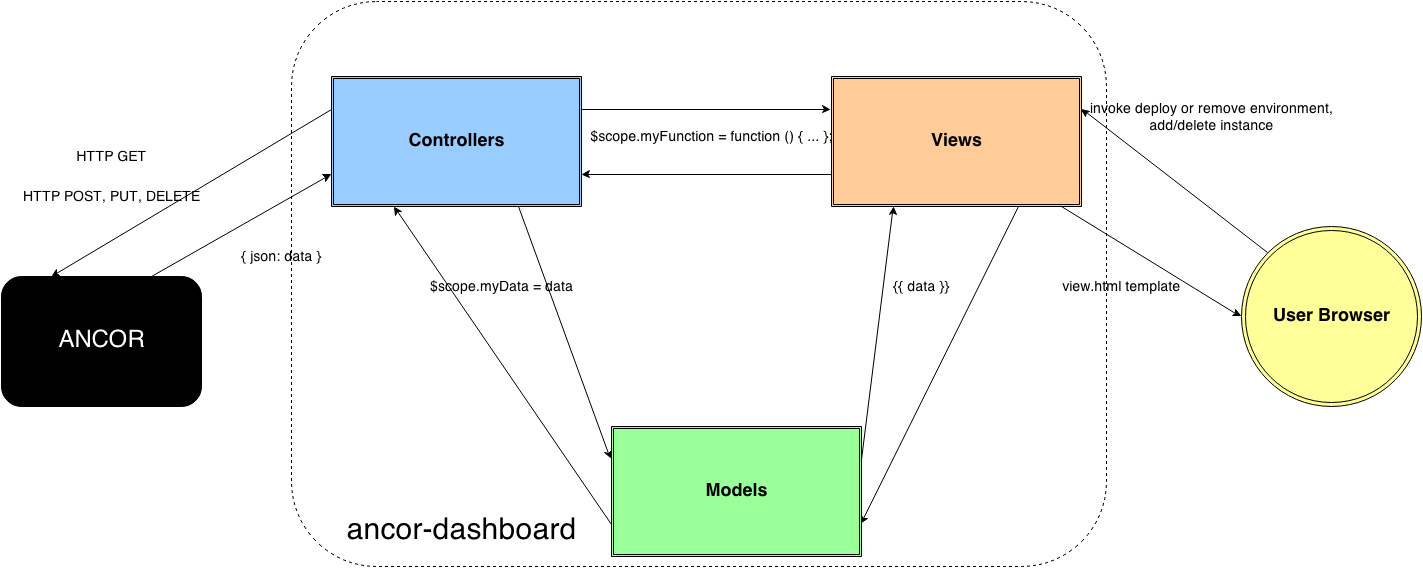
\includegraphics[height=2.8in]{figures/ad.png}

    \caption[\projectName{} Full Architecture
    ]{Full caption to appear below the Figure}

    \label{fullArchitecture}
\end{figure}

\section{Prototyping}
\label{makereference3.2}

Initially, this project was developed with Ruby on Rails. After a few months of development, it became clear that Ruby on Rails was a heavy framework to use for a project like this. Not only that, but because of the way Ruby on Rails works, it added an extra step to interact with \ancor{}. With Ruby on Rails, if a user wanted to make an API call to \ancor{} (like deploying a configuration file or viewing tasks), the user would have the browser talk to the Ruby on Rails server, and then that server would talk to \ancor{}. This added an extra step in the interaction between \projectName{} and \ancor.

To resolve this issue, I redid the framework in AngularJS. With AngularJS, the software is compiled to minified CSS and JavaScript and ran on the users machine directly. This compiled code will often be placed in an Apache or Nginx server to be served out to the user. In this case, there is no longer that extra medium required to talk to \ancor. Now the user can directly communicate with \ancor{} through their browser without needing to query a Ruby on Rails server first.

\section{\projectName{} Code Discussion}
\label{makereference3.3}

In this section, I will break down some of the major functionalities of \projectName{} and talk about how the code accomplishes those functionalities.

\subsection{REST over HTTP with AngularJS}

Earlier in chapter 2, I mentioned the idea of how \projectName{} communicates with \ancor{} with a concept called REST over HTTP. As mentioned before, REST has several different protocols to interface with: \emph{GET, PUT, POST, and DELETE}. But how exactly does that work within this project? Let's take a look at the Main controller to get a better idea of how this interaction works.

\begin{figure}[H]
  \begin{center}
    \renewcommand{\theFancyVerbLine}{
      \sffamily\textcolor[rgb]{0.5,0.5,0.5}{\scriptsize\arabic{FancyVerbLine}}}
    \begin{minted}[mathescape,
                   linenos,
                   numbersep=5pt,
                   gobble=2,
                   frame=lines,
                   framesep=2mm]{javascript}
    $http.get($rootScope.ancorIPAddress+'/v1').success(function(data) {
      $scope.version = data.version;
    });
    \end{minted}

  \end{center}
  \caption{\projectName{} using REST to ask \ancor{} what version it is.}
  \label{httpGET}
\end{figure}

\begin{figure}[H]
  \begin{center}
    \renewcommand{\theFancyVerbLine}{
      \sffamily\textcolor[rgb]{0.5,0.5,0.5}{\scriptsize\arabic{FancyVerbLine}}}
    \begin{minted}[mathescape,
                   linenos,
                   numbersep=5pt,
                   gobble=2,
                   frame=lines,
                   framesep=2mm]{html}
    <title>ANCOR {{version}} Dashboard</title>
    \end{minted}

  \end{center}
  \caption{Displaying a model variable within a view.}
  \label{modelView}
\end{figure}

In figure \ref{httpGET}, we have a simple HTTP GET call to \ancor{} that is retrieving the \emph{version} to display to the user on the dashboard. It queries the version number through a URL, and then \ancor{} responds with a json formatted data set. In this case, \ancor{} responds with the version number. In the controller we set that version to a model variable to be displayed on the view as seen in figure \ref{modelView}. The double brackets in AngularJS represent an evaluation. Because the variable version exists within the \$scope model, the view is able to display that value within HTML to the user. If no data is returned from \ancor{} in the controller,  the \emph{version} model variable will be empty and the evaluation will be left blank when the view is compiled.

\begin{figure}[H]
  \begin{center}
    \renewcommand{\theFancyVerbLine}{
      \sffamily\textcolor[rgb]{0.5,0.5,0.5}{\scriptsize\arabic{FancyVerbLine}}}
    \begin{minted}[mathescape,
                   linenos,
                   numbersep=5pt,
                   gobble=2,
                   frame=lines,
                   framesep=2mm]{javascript}
    $scope.addNewRole = function (roleSlug) {
      var url = $rootScope.ancorIPAddress+'/v1/instances',
          newRole = { 'role': roleSlug };
      $window.alert('New role ' + roleSlug + ' added!');
      $http.post(url, newRole);
      $route.reload();
    };
    \end{minted}

  \end{center}
  \caption{Code from the Main controller to add a new role to \ancor{} with an HTTP POST call.}
  \label{httpPOST}
\end{figure}

In figure \ref{httpPOST}, we have an example of an HTTP POST call to \ancor{}. In this case, this function is invoked when a user is interested in adding a new role through the role dropdown generated on the main page. First it builds the correct URL with a json data key value structure. It alerts the user that the invocation has started, and then sends the json data to the specified URL. \ancor{} will then take over from there, and the page is reloaded.

\subsection{D3 Network Graph}

On the main view of the dashboard, we have a dynamically generated network graph that uses D3js. This can be seen in figure \ref{networkGraph}. The initial graph drawing code was modified from one of the numerous D3js examples on the main website. However the code has been modified to work within the project itself. For example, to generate the nodes on the network, it must take a specially formed set of data from the Main controller. The main controller first does an HTTP GET call to retrieve all of the instances. Within this json on each instance, there is a \emph{depends\_on} attribute that is used to get what each node depends on and interacts with. A json object is then created with the source name, each sources dependency (or target in this case), the type of dependency (this will determine the color and style of the line with css), and the source ID. This data set is then passed into the method located in \emph{forced-graph.js} that generates the entire network graph.

The network graph code also defines how large each node circle will be, the length between connections, the color and size of the text used, and so on. Everything about the network graph is customizable here. Another modification to the network graph script was preventing the graph from jumping around when first loaded. Many D3js examples have very active elements when first loaded, almost like bouncy balls being released into a gymnasium. There is a simple method near the bottom that skips this activity so the graph looks more static on first load. This does not however prevent the user from dragging nodes around and moving the network graph on the page.

It has an event method for when a user selects one of the nodes. At the moment, this method only prints the node name and id to the JavaScript console. However in the future this method will be used for more than just that. See the future work section for more information.

\subsection{ACE Editor}

% image of ace editor?

The ACE Editor is an important part of the configuration writing process with \projectName{}. Thanks to the angular-ui library, integrating the ACE Editor is extremely easy. In figure \ref{aceEditorHTML}, we can see that adding a new editor is as easy as making a simple div tag with a few options defined. We give this div a specific id so that the controller knows which div to apply to.

\begin{figure}[htb]%t=top, b=bottom, h=here

    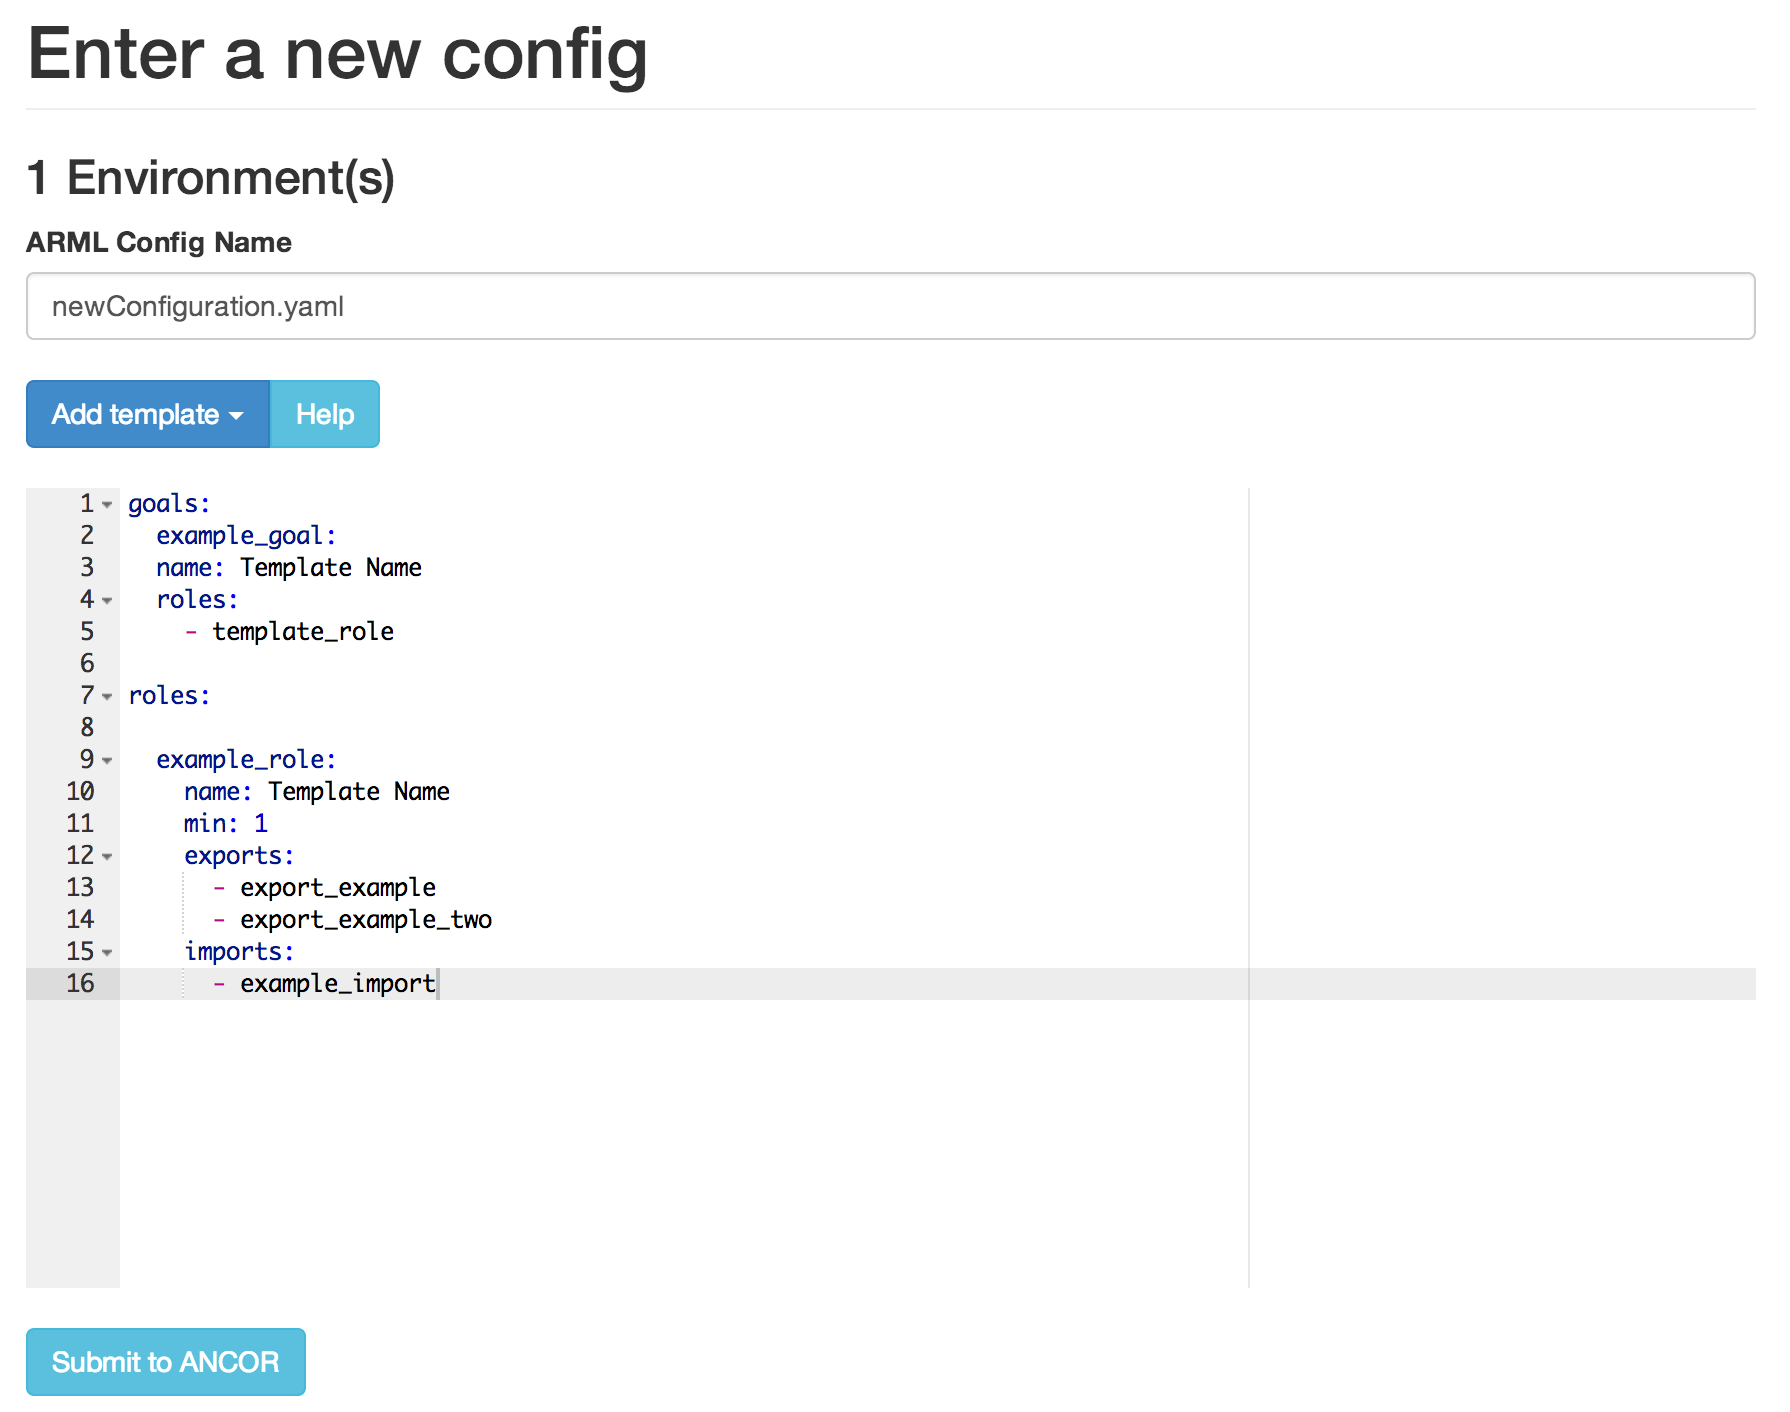
\includegraphics[height=5.0in]{figures/ace-editor-example.png}

    \caption[ACE Editor example
    ]{An example of what the ACE Editor looks like with a sample config file.}

    \label{aceEditorSample}
\end{figure}

Next with angular-ui, we pass in different configuration options to customize ACE. For example, the configuration files that \ancor{} uses are of the yaml syntax, thus we tell ACE to use yaml syntax highlighting for anything within the editor. useWrapMode is a standard text editing feature that prevents users from having to scroll side to side while typing up a document. Finally the two functions onLoad and onChange are functions defined by angular-ui's ACE package for when the editor first loads and when someone makes a change within the editor. These options are just the names of the functions from within the controller. An example of how the onChange and onLoad functions work can be seen in figure \ref{aceEditorOnChange}.

\begin{figure}[H]
  \begin{center}
    \renewcommand{\theFancyVerbLine}{
      \sffamily\textcolor[rgb]{0.5,0.5,0.5}{\scriptsize\arabic{FancyVerbLine}}}
    \begin{minted}[mathescape,
                   linenos,
                   numbersep=5pt,
                   gobble=2,
                   frame=lines,
                   framesep=2mm]{html}
    <div id="editor" ui-ace="{
      mode: 'yaml',
      useWrapMode: true,
      onLoad: loadConf,
      onChange: confChange
      }">
    </div>
    \end{minted}

  \end{center}
  \caption{Initializing the ACE Editor with angular-ui.}
  \label{aceEditorHTML}
\end{figure}

\begin{figure}[H]
  \begin{center}
    \renewcommand{\theFancyVerbLine}{
      \sffamily\textcolor[rgb]{0.5,0.5,0.5}{\scriptsize\arabic{FancyVerbLine}}}
    \begin{minted}[mathescape,
                   linenos,
                   numbersep=5pt,
                   gobble=2,
                   frame=lines,
                   framesep=2mm]{javascript}
    $scope.loadConf = function(_editor) {
      var _session = _editor.getSession();
      _session.setUndoManager(new ace.UndoManager());
    };

    $scope.confChange = function(e, _editor) {
      $scope.submitData = _editor.getValue();
    };
    \end{minted}

  \end{center}
  \caption{Two examples that help operate the ACE Editor. loadConf is what initializes the editor, while confChange keeps the configuration model variable up to date as a user writes their configuration file.}
  \label{aceEditorOnChange}
\end{figure}

\subsection{Table Filtering with AngularJS}

One of the advantages of using AngularJS is how simple they have made implementing complex features in HTML and JavaScript. One example of this is the search box that exists on the Main and Tasks view for filtering the large tables of data from \ancor{}. This consists of only a few components in the HTML template. The first one is the textbox. From figure \ref{filterTextSearch}, you can see the input text box tag with an ng-model attribute. This model variable is what keeps track of the input from the user.

The only other element to this powerful search function is the filter attribute when AngularJS builds the Task or Instance rows within the table. Looking at line 5 of figure \ref{filterTextSearch}, the final element in ng-repeat is \emph{filter:searchText}. This means if a user starts typing and modifying the model searchText, it will filter the results in the table automatically. This is a very powerful feature that only required a few lines of code thanks to AngularJS.

\begin{figure}[H]
  \begin{center}
    \renewcommand{\theFancyVerbLine}{
      \sffamily\textcolor[rgb]{0.5,0.5,0.5}{\scriptsize\arabic{FancyVerbLine}}}
    \begin{minted}[mathescape,
                   linenos,
                   numbersep=5pt,
                   gobble=2,
                   frame=lines,
                   framesep=2mm]{html}
    . . .
    <input type="text" placeholder="Search tasks..." 
      class="form-control" ng-model="searchText" />
    . . .
    <tr ng-repeat="task in tasks | orderBy:predicate:reverse | filter:searchText">
    . . .
    \end{minted}

  \end{center}
  \caption{An example of how AngularJS easily creates a filtering search box within a template view.}
  \label{filterTextSearch}
\end{figure}

\section{Component Breakdown}
\label{makereference3.4}

In this section, I will talk about the different components of \projectName. I will cover everything that exists in the controller as well as the viewmodel for each component.

\subsection{Main}

The main component of \projectName{} is the root route of the project. This means when a user first visits the main URL for \projectName{}, they will be presented with this view. This is the view in charge of displaying information about instances from \ancor{}. Once a user visits Main, the controller will then query \ancor{} through REST for its current version, all of the goals, all of the roles, and all of the instances.

These HTTP GET calls will then save the relevant information in the \$scope model for the view to use. Querying goals will get the name of the current deployment. This name is saved and shown as a title on the front page. Roles are queried for the add instance dropdown. Each role slug is saved so a user can select one from a dynamically generated dropdown.

With the call against \ancor{} instances, there is a bit of extra logic to keep track of each instances current stage and planned stage. The current stage is what is displayed to the user on the front page. It also shows how many total instances there are. Finally, data is saved and sent to the network graph generation script. This information is a set of data that shows how all of the instances are related to each other.

Two functions exist in this controller to replace and delete instances. They both are given an instance id, form the correct URL, and then make the appropriate REST HTTP call (either POST or DELETE) to \ancor{}.

There is a helper function to determine which label to apply to an instances state from the Instance table. This is needed so that the HTML template file can stay as simple as possible and let the controller do all of the logic for which class label to apply.

Finally, there are several functions in charge of showing the modal popup when a user is interested in viewing more information about each instance. These modal functions are mostly used by angular-ui's Bootstrap package.

\subsection{Env}

The Environment component is used to show the current deployment from \ancor{}. When this route is first loaded, the controller queries \ancor{} for its version and all of the current environments. At the moment, \projectName{} only supports one deployment, so we grab the first environment in the data returned.

The main function in this controller is the ability to delete the given environment. When the user clicks the delete button from the view, it passes the environment id to the controllers \emph{deleteEnv} function. This function then builds the correct URL with the id appended onto the end, and makes the HTTP DELETE call to \ancor{}.

Environment also has a helper function to determine if the delete button should be disabled or not. If the environment is locked, the button will become greyed out so the user cannot click on it. Otherwise, the button will be enabled.

\subsection{Tasks}

The Tasks view is what is in charge of displaying all current \ancor{} Tasks. When the Tasks view is first loaded up by the user, the controller then queries \ancor{} for its current version and all of the tasks. The HTTP GET for Tasks is different from other controllers however because it needed to be able to be refreshed constantly so a user could see the tasks progress. For this to happen, the HTTP GET call was wrapped up in a function within the controller. However since there is a call to that function \$scope.getData(), it is invoked initially when the route is loaded. Another way to update the task list is to select the \emph{Refresh} button located right above the filtering search box. Finally like the other endpoints, Tasks has a helper function to determine the label for each Tasks state.

\subsection{Deploy}

The Deploy view is where the user can write their own configruation file and deploy it directly to \ancor{}. When the Deploy route is loaded, it will query \ancor{} for its version and the current deployed environment. The environment is required just so the user can know if any environments are currently deployed to prevent any overlap.

roleTemplate and goalTemplate are what generates the template text for the configuration within the ACE Editor. It simply uses an already made string template and inserts it where the curser is at within ACE.

There are two functions that relate directly to the ACE editor API. The first one is loadConf, which is in charge of initializing the editor. The next one is called confChange. This function is in charge of keeping the configuration data model up to date within Deploys model.

The deploy function takes the current data from the ACE editor and constructs a message to be sent off to \ancor{}. Before this happens, it builds two urls: A URL for planning the new deployment which will contain all of the configuration file data, and a URL for telling \ancor{} to begin the deployment. Once these URLS are created and the configuration data is saved, the deploy function makes these two HTTP PUT and POST calls (in that order) to \ancor{}.

The modal for Deploy uses all of the angular-ui conventions for displaying a modal to the users. It displays an example configuration, and gives some help text to help the user understand how to write a configuration file.
